% This is samplepaper.tex, a sample chapter demonstrating the
% LLNCS macro package for Springer Computer Science proceedings;
% Version 2.20 of 2017/10/04
%
% \documentclass[runningheads]{llncs}
\documentclass[
	fontsize=11pt, % Base font size
	twoside=false, % Use different layouts for even and odd pages (in particular, if twoside=true, the margin column will be always on the outside)
	open=any, % If twoside=true, uncomment this to force new chapters to start on any page, not only on right (odd) pages
	secnumdepth=1, % How deep to number headings. Defaults to 1 (sections)
]{kaobook}
\setchapterstyle{kao} % Choose the default chapter heading style
\usepackage{kaobiblio}
\bibliography{references.bib}
%
\usepackage{graphicx}
\usepackage{amsmath}
\usepackage{amssymb}
\usepackage{gensymb}
\usepackage{booktabs}
\usepackage{multirow}

\newcommand{\TP}{\operatorname{TP}}
\newcommand{\TN}{\operatorname{TN}}
\newcommand{\FP}{\operatorname{FP}}
\newcommand{\FN}{\operatorname{FN}}

\usepackage[misc,geometry]{ifsym}

% Used for displaying a sample figure. If possible, figure files should
% be included in EPS format.
%
% If you use the hyperref package, please uncomment the following line
% to display URLs in blue roman font according to Springer's eBook style:
% \renewcommand\UrlFont{\color{blue}\rmfamily}

\begin{document}
%
\renewcommand*{\thechapter}{\Roman{chapter}}
\addtocounter{chapter}{6}
\chapter{Feature learning for class separability applied to COVID-19 chest X-ray case study}

\begin{widepar}
  \begin{kaobox}[frametitle=Source]
    Charte, D., Sevillano-García, I., Lucena-González, M. J., Martín-Rodríguez, J. L., Charte, F., \& Herrera, F. (2021, September). Slicer: Feature Learning for Class Separability with Least-Squares Support Vector Machine Loss and COVID-19 Chest X-Ray Case Study. In \textit{International Conference on Hybrid Artificial Intelligence Systems} (pp. 305-315). Springer, Cham.
\end{kaobox}
\end{widepar}
%
% \titlerunning{Slicer: Feature Learning for Class Separability with LSSVM Loss}
% If the paper title is too long for the running head, you can set
% an abbreviated paper title here
%
% \author{David Charte\inst{1}\textsuperscript{(\Letter)}\orcidID{0000-0002-4830-9512} \and 
% Iv\'an Sevillano-Garc\'ia\inst{1}\orcidID{0000-0002-5029-9106} \and 
% Mar\'ia Jes\'us Lucena-Gonz\'alez\inst{3}\and 
% Jos\'e Luis Mart\'in-Rodr\'iguez\inst{3}\and
% Francisco Charte\inst{2}\orcidID{0000-0002-3083-8942} \and
% Francisco Herrera\inst{1}\orcidID{0000-0002-7283-312X}}

% %
% \authorrunning{D. Charte et al.}
% % First names are abbreviated in the running head.
% % If there are more than two authors, 'et al.' is used.
% %
% \institute{Department of Computer Science and Artificial Intelligence, Andalusian Research Institute in Data Science and Computational Intelligence (DaSCI), University of Granada, Granada, Spain.
% \\\email{\{fdavidcl,isevillano\}@ugr.es,herrera@decsai.ugr.es}\and
% Department of Computer Science, Andalusian Research Institute in Data Science and Computational Intelligence (DaSCI), University of Ja\'en, Ja\'en, Spain.
% \\\email{fcharte@ujaen.es}\and
% Hospital Universitario Cl\'inico San Cecilio de Granada, Granada, Spain
% \\\email{mjlucgon@gmail.com,joseluismartin.rx@hotmail.com}}
% %
% \maketitle              % typeset the header of the contribution
%
\section*{Abstract} % limits 150-250 words
Datasets from real-world applications usually deal with many variables and present
difficulties when modeling them with traditional classifiers. There is a variety of feature
selection and extraction tools that may help with the dimensionality problem, but most of them
do not focus on the complexity of the classes. In this paper, a new autoencoder-based model
for addressing class complexity in data is introduced, aiming to extract features that present
classes in a more separable fashion, thus simplifying the classification task. This is possible thanks to a combination of the standard reconstruction error with a least-squares support vector machine loss function. This model is
then applied to a practical use case: classification of chest X-rays according to the presence
of COVID-19, showing that learning features that increase linear class separability can boost classification performance. For this purpose, a specific convolutional autoencoder architecture has been designed and trained using the recently published COVIDGR dataset. The proposed model is evaluated by means of several traditional classifiers and metrics, in order to establish the improvements caused by the extracted features. The advantages of using a feature learner and traditional classifiers are also discussed.
\section*{Keywords}Feature learning  - Class separability - Autoencoders.
% \end{abstract}

\section{Introduction}\label{sec.intro}

Data classification \cite{Aggarwal2015} is one of the most studied problems in machine learning, and is applicable in many real-world contexts such as medicine, banking, robotics, natural sciences and other industries. Class complexity \cite{pascual2021revisiting,basu2006data} is a term which encompasses all the intrinsic traits in data that can hinder the performance of a classifier. There are several categories of metrics that can be used to gauge the complexity of a dataset: feature overlap, linearity, neighborhoods, dimensionality, class balance and network properties. Datasets that present high levels of complexity in some of these categories have been shown to cause poor classifier performance \cite{luengo2011addressing}.

When it comes to addressing data complexity during a preprocessing \cite{garcia2015data} phase, several specific methods can be found on the literature, but they usually tackle high dimensionality (feature selection and extraction methods) and class imbalance (resampling methods). Little research has been published on how to address other complexity types during a preprocessing phase and most of it is centered around feature selection \cite{zhang2013divergence,wang2008feature}.

In this work, we present Slicer (supervised linear classifier error reduction), an automatic feature extractor designed with linear class separability in mind. It is based on an autoencoder (AE) model \cite{charte-tutorial}, using a special loss function inspired by least-squares support vector machines (LSSVM) \cite{suykens1999least}. The objective of this model is to learn an alternative representation for each instance where classes are more easily distinguishable. Once trained, the model is able to project any new instance onto the learned feature space without knowing its class. This allows to work with compact representations of the samples instead of the original, high-dimensional ones, in a way that facilitates the work of traditional classifiers, which are usually hindered by high dimensionality \cite{aggarwal2001surprising,beyer1999nearest} unless they specifically select features internally. Extracting features can also help when it is necessary to combine variables from different sources (e.g. images and clinical data), and working with traditional classifiers makes it easier to understand the decision-making process.

The proposed model is applied in a specific use case, aiming both to analyze the level of performance that could be gained and to open new possibilities for combination of imagery and other data, as well as interpretability of classifiers. The chosen application is recognition of COVID-19 in chest X-ray images, using the COVIDGR dataset \cite{9254002} for this purpose. The fitness of the set of features learned by Slicer is evaluated by means of classification metrics using several standard classifiers and is compared against using a basic AE and learning from the original, unmodified features. The results show a noticeable advantage of the Slicer-generated variables except when using support vector machines as classifier, even though specific traits of this dataset such as ``apparently negative'' positive samples might affect the learned representation.

The rest of this document is organized as follows. Section~\ref{sec.method} describes the new feature learner named Slicer. Afterwards, Section~\ref{sec.exp} outlines the main aspects of the experimentation, including the dataset and the evaluation strategy. Section~\ref{sec.res} discusses the results obtained in the experimentation above and, lastly, Section~\ref{sec.conc} draws some conclusions.

\section{Class-informed autoencoder for complexity reduction}\label{sec.method}

This section is dedicated to introducing a new model designed to learn features with improved class separability. The proposed model, Slicer, is based on the minimization of the error of a linear classifier, at the same time that it attempts to maximize its reconstruction abilities. As a result, the learned features are influenced both by the overall information within the data as well as their relation to the class.

\subsection{Autoencoder fundamentals}

An AE is an artificial neural network that is trained to reconstruct the inputs at its output \cite{charte-tutorial}. It includes a certain bottleneck where the representation of the data is somehow restricted: e.g. it is lower dimensional, more sparse or robust against noise. This prevents the AE from simply copying the input instance throughout the network. Instead, an encoder $f$ learns a new representation for the data while a decoder $g$ must be able to recover the original features. This transformation is learned by optimizing the reconstruction error $\mathcal J_{\operatorname{RE}}(x,(g\circ f)(x))$ which typically measures a distance between the original samples and their reconstructions, but different penalties and regularizations can allow to influence other aspects of the learned representation.

AEs are usually unsupervised tools, in the sense that they do not receive any information about the labels of the data nor the desired encodings for each instance. Their learning mechanism is, as a result, self-supervised \cite{liu2020self}. This means that they can be applied in many contexts where label information is not necessarily available or just partially so: anomaly detection, semantic hashing, data compression, among others \cite{CHARTE202093}. Nonetheless, some AEs do use label information~\cite{makhzani2015adversarial}, even though the objective is other than learning more separable features. Our objective is to regularize an AE so that it learns from the class labels during training, but does not need them during the prediction phase, and thus facilitates classification tasks.

\subsection{Slicer model: the loss function}

Slicer is an AE model regularized by a special penalty function which takes class separability into account. In order to do this, an additional component is introduced to simultaneously fit a LSSVM to the encoded samples as well as evaluate the encoding based on the fitness of said classifier.

Figure~\ref{fig:slicerdiag} shows a diagram with the main components of Slicer. $f$ represents the encoder, which is a neural network that transforms the inputs onto encodings. $g$ refers to the decoder, a similar network whose objective is to reconstruct the original data inputs out of the encodings. These encodings are also fed to a single fully connected layer with no activation function, which acts as the support vector machine. Each of the decoder and this last layer are evaluated with their loss functions: the reconstruction error and the LSSVM minimization objective, respectively.

\begin{figure}
    \centering
    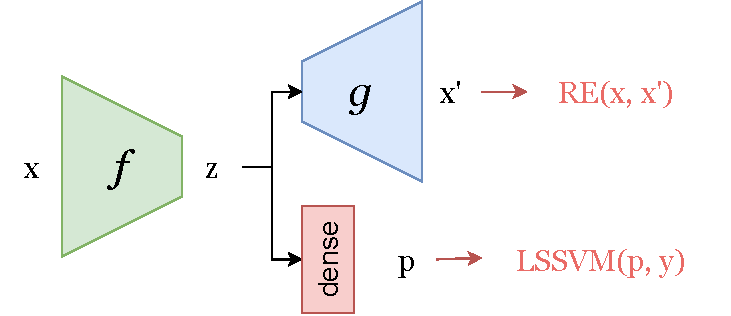
\includegraphics[width=0.6\linewidth]{slicer.pdf}
    \caption{Schematic illustration of the Slicer model}
    \label{fig:slicerdiag}
\end{figure}

The reconstruction error chosen for the purposes of modeling input samples is cross entropy: a measure of disagreement between two probability distributions, for the case of Bernoulli distributions. It is usually the better option when all values in each instance are in the $[0,1]$ interval.  Its formulation for $n$ instances with $k$ variables is shown in Eq.~\ref{eq.crossent}.
\begin{align}
\begin{split}\label{eq.crossent}
    \mathcal J_{\mbox{RE}}(x,\theta)=-&\frac{1}{nk}\sum_{i=1}^n\sum_{j=1}^k x^{(i)}_j \log\left[ (g\circ f)\left(x^{(i)}\right)_j\right] +\\& \left(1-x^{(i)}_j\right)\log\left[1-(g\circ f)\left(x^{(i)}\right)_j\right]~.
\end{split}
\end{align}
If the variables are not scaled to the $[0,1]$, other reconstruction errors like the mean squared error could be used.

For its part, the LSSVM objective assumes that labels are in $\{-1,1\}$ and is simply a sum of quadratic errors $e_i^2$ subject to the equality constraint $1-e_i=y^{(i)}-w^Tf\left(x^{(i)}\right)+b$, resulting as formulated in Eq.~\ref{eq.lssvm}.
\begin{equation}\label{eq.lssvm}
    \mathcal J_{\mbox{LSSVM}}(x,y,\theta)=\frac\mu 2w^Tw+\frac \zeta 2\sum_{i=1}^n \left(y^{(i)}-w^Tf\left(x^{(i)}\right)+b\right)^2~.
\end{equation}
In the previous equation, $f$ usually refers to the kernel used in the model but, in this case, it represents the encoder of the neural network. $w$ holds the weights of the SVM, which are associated to a penalty with coefficient $\mu$. The term that compares classes ($y$) to the LSSVM output is weighted by $\zeta$.

The resulting loss function for the Slicer model is the sum of both the reconstruction error and the LSSVM loss:

\begin{equation}
    \mathcal{J}(x,y,\theta)=\mathcal J_{\mbox{RE}}(x,\theta)+\mathcal J_{\mbox{LSSVM}}(x,y,\theta)
\end{equation}

\section{Experimental framework}\label{sec.exp}

The objective of this experimentation is to apply the proposed complexity reduction method in a real world practical case. In particular, we aim to improve the performance of simple classifiers when dealing with a chest X-ray image dataset for COVID-19 classification. This would open several promising research lines, such as the combination of these extracted features with other clinical and laboratory variables or the possibility of using easily interpretable classifiers with the generated features.

\subsection{COVIDGR dataset}

The COVIDGR dataset of X-ray chest images was introduced in \cite{9254002}. These images were collected under a collaboration with expert radiologists of the Hospital Universitario San Cecilio in Granada, Spain. In total, 852 images were annotated under a strict protocol: positive images correspond to patients who have been tested positive for COVID-19 using RT-PCR within a time span of at most 24h between the X-ray image and the test. Every image was taken using the same type of equipment and always with the posterior-anterior view. It is important that all images are consistent since, otherwise, classifiers could find cues to distinguish COVID-positive samples from negative ones different from the intended aspects of the X-ray that characterize the pneumonia associated to the disease \cite{MAGUOLO20211}. Figure~\ref{fig:covidgrsamples} includes one positive example and a negative one. 

\begin{figure}
    \centering
    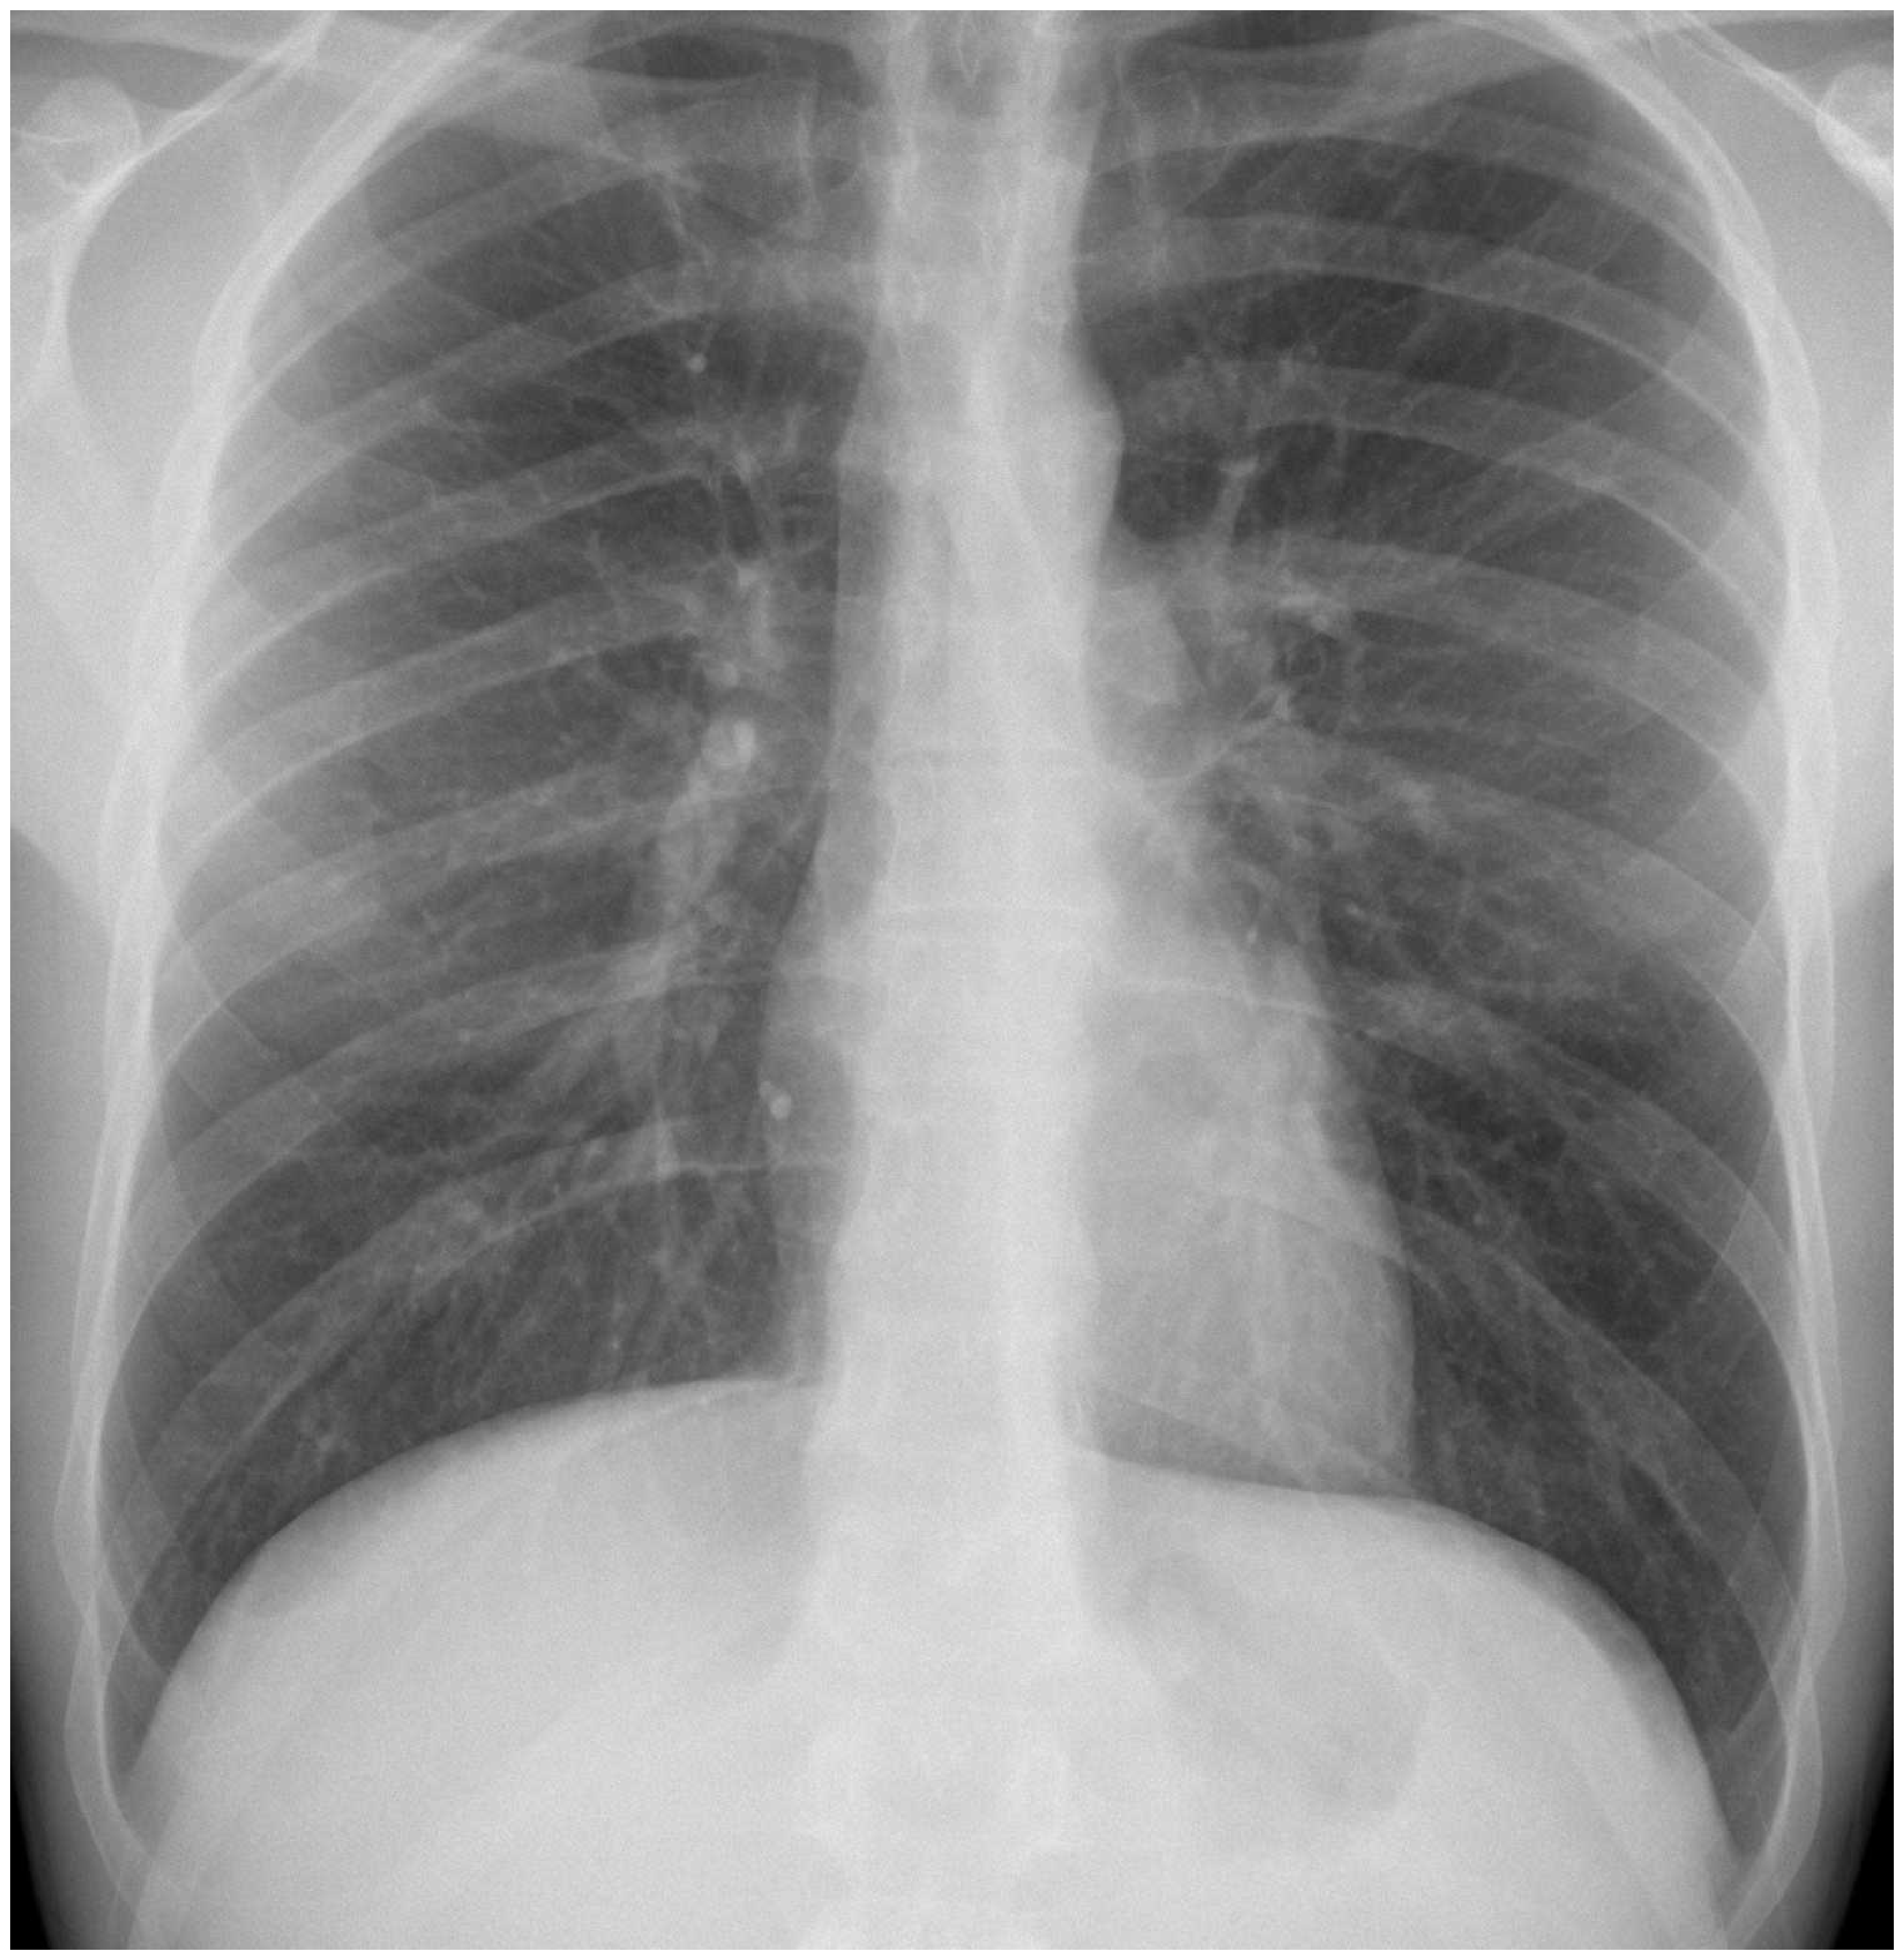
\includegraphics[height=.33\linewidth]{Negativa-min.eps}~~
    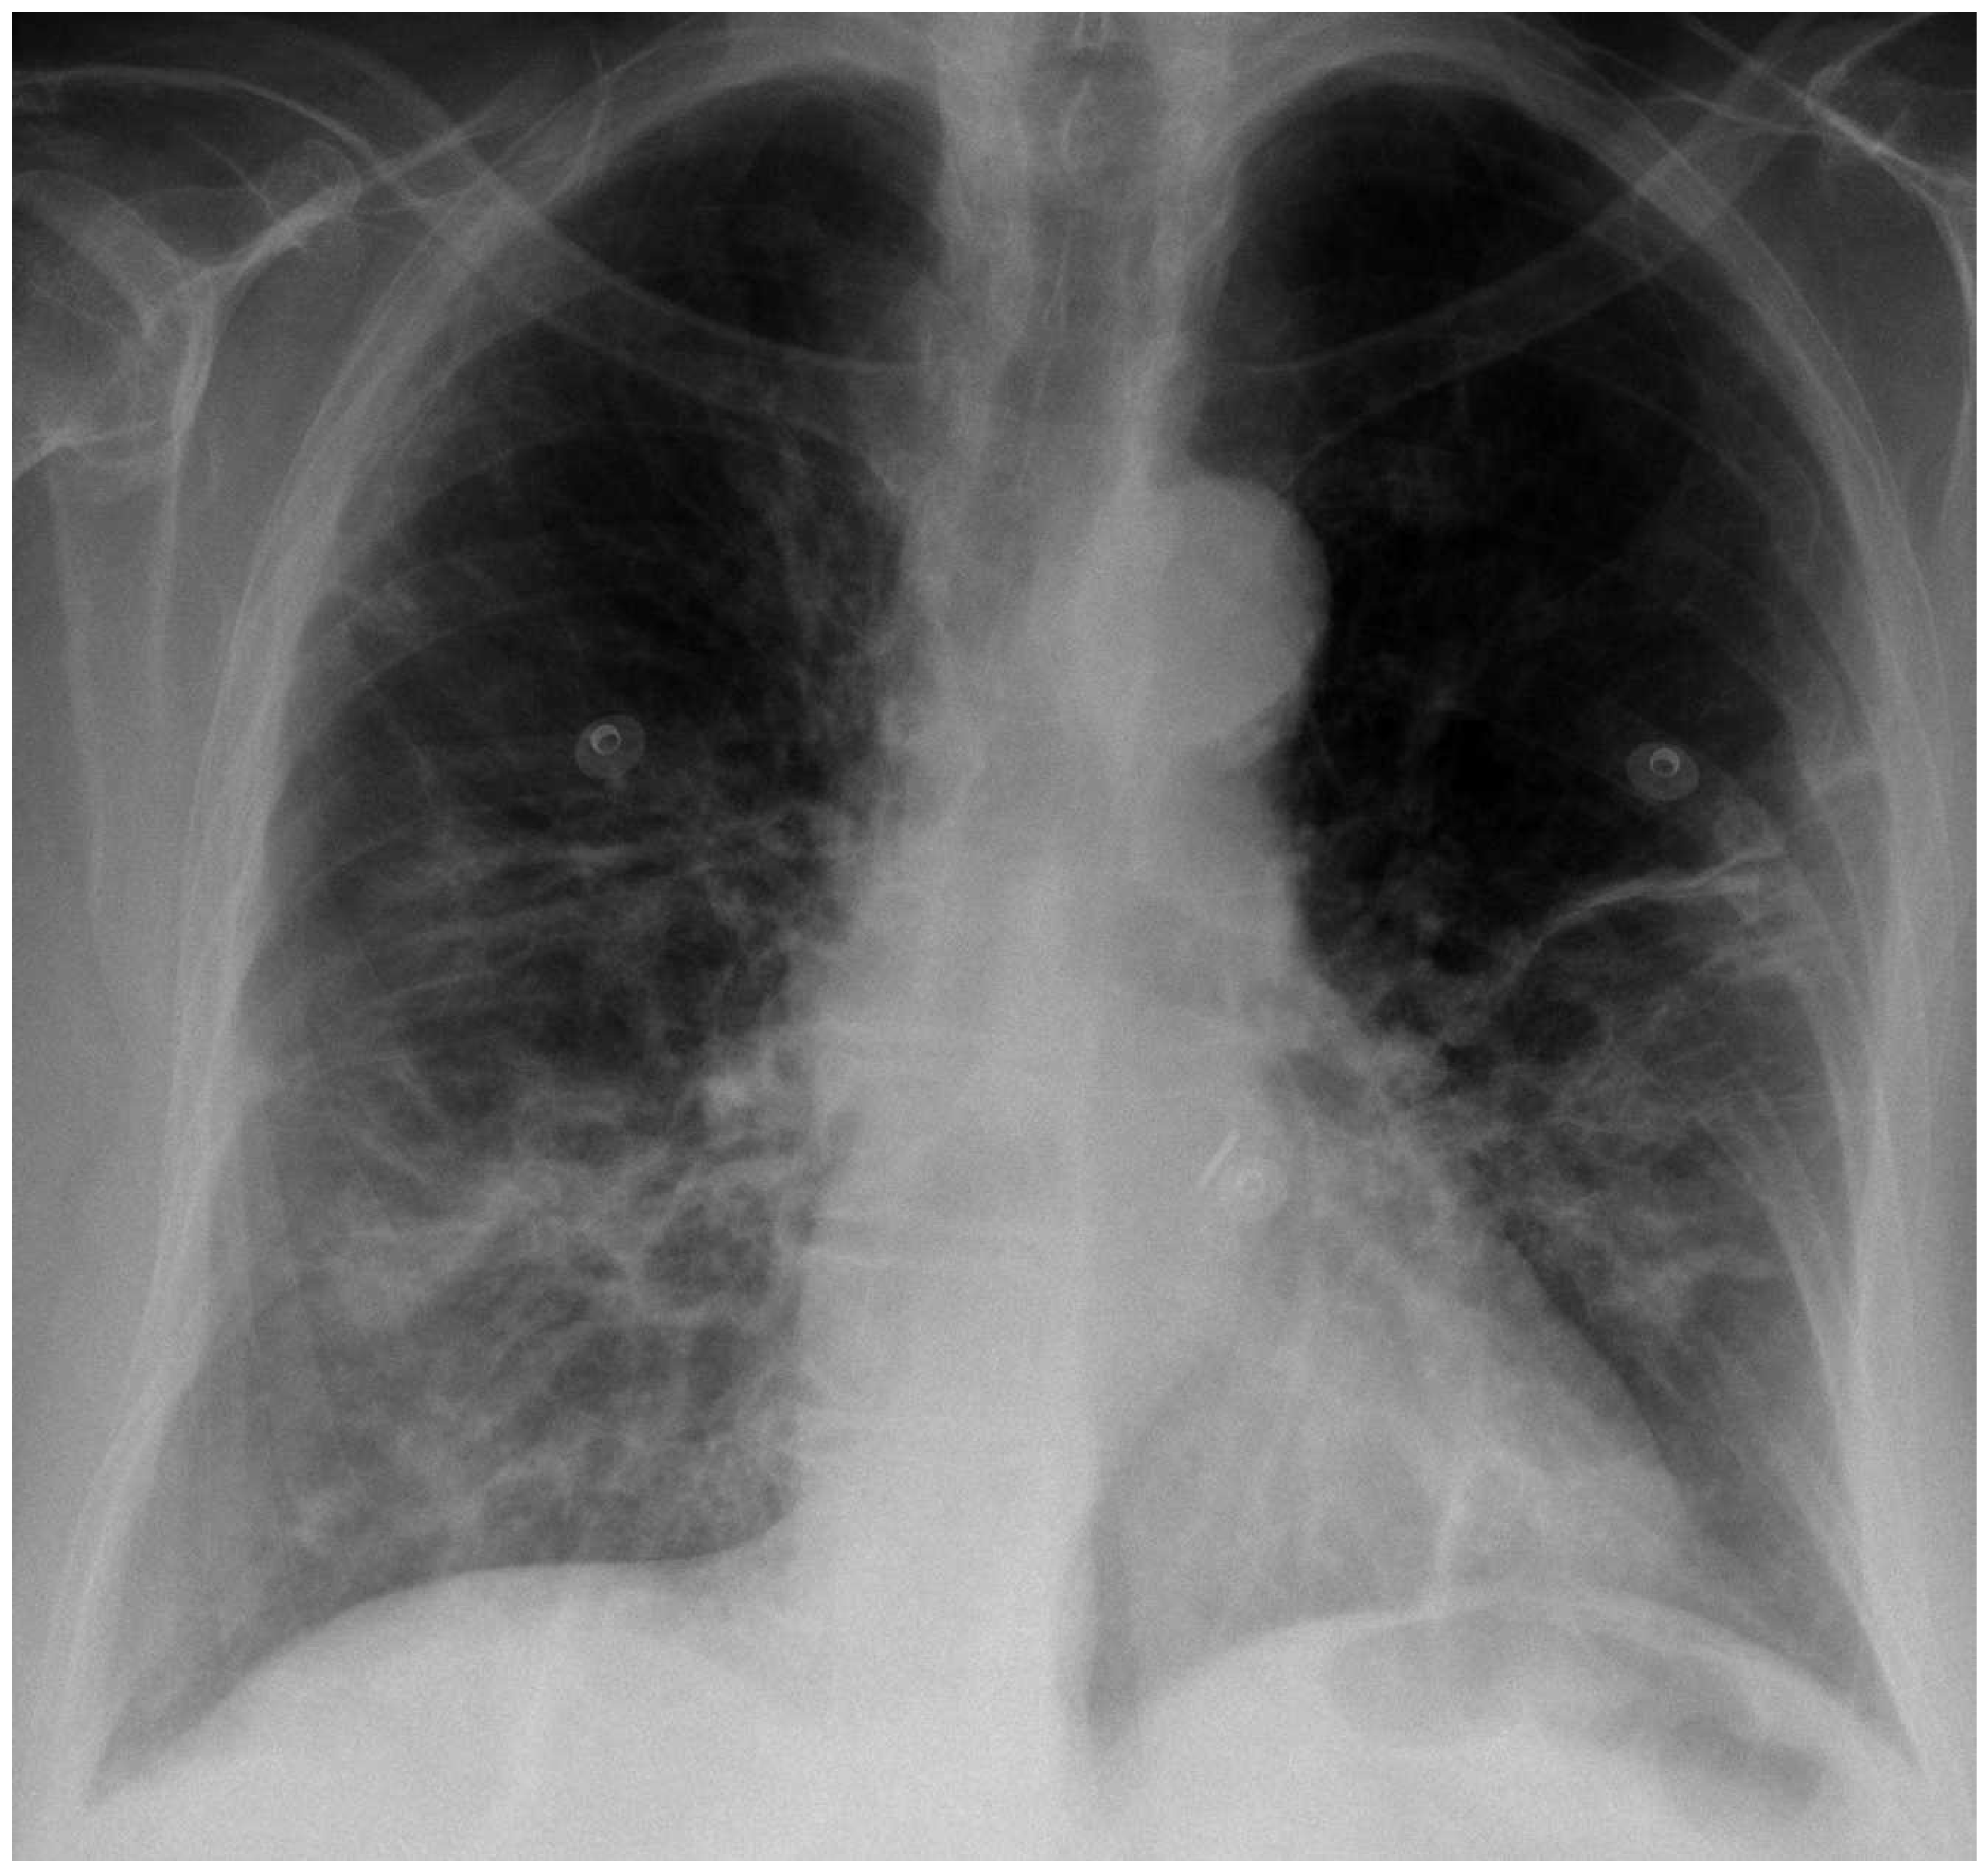
\includegraphics[height=.33\linewidth]{Severa-min.eps}
    
    \caption{A negative sample (left) and a positive one (right)}
    \label{fig:covidgrsamples}
\end{figure}

More information about class distribution is provided in Table~\ref{tab:classdist}. In the following experiments, the exact same partitions used in \cite{9254002} are employed, in order to ease comparisons with previous results.


\begin{table}[htbp]
    \centering
    \begin{tabular}{lrllr}
    \toprule
        \bfseries class & \bfseries \#images &~ &\bfseries  severities \\
        \midrule
         negative & 426 && &\\\midrule
         \multirow{4}{*}{positive} & \multirow{4}{*}{426} && Normal-PCR+& 76\\
         &&& Mild& 100\\
         &&& Moderate& 171\\
         &&& Severe& 79\\
         \bottomrule
    \end{tabular}
    \caption{Class distribution in COVIDGR dataset. Normal-PCR+ refers to X-rays where COVID-19 was not detected by the experts but the patients tested positive.}
    \label{tab:classdist}
\end{table}


\subsection{Evaluation strategy}

Since the final objective of the proposed model is to improve classification performance, the evaluation framework will consist in a variety of simple classifiers that will be trained with either the original features or the encoded ones. Standard classification metrics will be computed using the predictions over test subsets. A 5-fold cross validation scheme will be applied 5 times for a total of 25 train-test runs, so as to prevent errors from statistical chance. Table~\ref{tab:eval} lists the available feature sets and every classifier and evaluation metric included in the experiment. Each column is independent, in the sense that every feature set has been tested with each one of the classifiers and the performance has always been assessed with all four metrics.

\begin{table}[htbp]
    \centering
    \begin{tabular}{lllc}
    \toprule
         \bfseries Feature sets~~ &\bfseries Classifiers &  \multicolumn{2}{l}{\bfseries Evaluation metrics} \\\midrule
         Original&Decision tree (DT) & Accuracy& \(\displaystyle\frac{\TP+\TN}{\TP+\TN+\FP+\FN}\) \\
\addlinespace
         Basic AE&$k$ nearest neighbors (kNN) & Precision& \(\displaystyle\frac{\TP}{\TP+\FP}\) \\
\addlinespace
         Slicer&Support vector machine (SVM)~~ & Recall& \(\displaystyle\frac{\TP}{\TP+\FN}\) \\
\addlinespace
         &Gaussian process (GP) & F1-score& \(\displaystyle\frac{2\cdot\operatorname{Precision}\cdot\operatorname{Recall}}{\operatorname{Precision}+\operatorname{Recall}}\) \\
     \bottomrule
    \end{tabular}
    \caption{Evaluation framework: available feature sets, tested classifiers and evaluation metrics. TP, TN, FP and FN denote true positives, true negatives, false positives and false negatives, respectively.}
    \label{tab:eval}
\end{table}
\vspace{-1em} 

\subsection{Architecture of the Slicer model used with the COVIDGR dataset}

The proposed Slicer model has been implemented in the Python language on top of the Tensorflow \cite{tensorflow2015-whitepaper} library. Since the model needs to deal with image data, the specific architecture makes use of convolutional layers for the encoder and deconvolutional (or transposed convolutional) layers for the decoder.

More specifically, most of the AE is composed of residual blocks such as the ones in the ResNet-V2 architectures \cite{he2016identity}, as can be seen in Figure~\ref{fig:architecture}. The left side of this diagram shows the detailed architecture of the AE-based model, with the encoder ranging from the input to the dense layer with 128 units, and the decoder from there to the last deconvolutional layer. The classification component consists in the fully connected (dense) layer that maps the encoding to one variable and is then connected to the LSSVM loss. The overall loss is simply the sum of both error measures, as explained above. 

\begin{figure}[htbp]
    \centering
    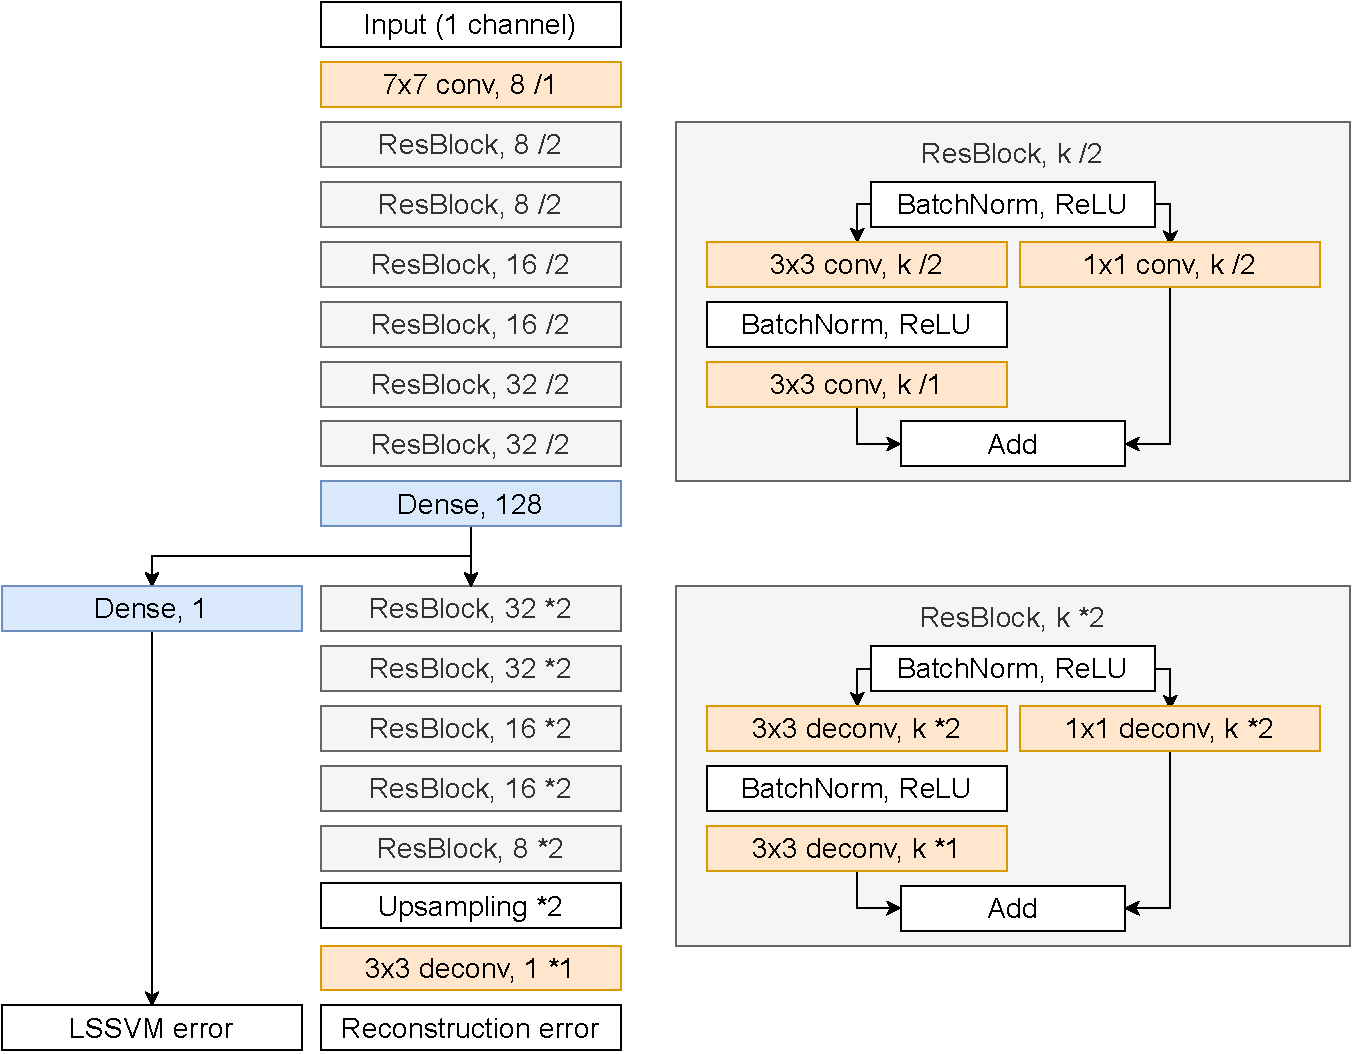
\includegraphics[width=.9\linewidth]{slicercovid.pdf}
    \caption{Structure of the Slicer model used with the COVIDGR dataset. Each convolutional and deconvolutional layer is followed by the number of filters as well as an indication of the stride: /2 indicates a stride of 2 for a convolutional layer (the side of the image is halved), and *2 indicates a stride of 2 for a deconvolutional layer (the side of the image is doubled). Each of the residual blocks unrolls like the corresponding diagram on the right.}
    \label{fig:architecture}
\end{figure}

Using the previous architecture, a model was trained for each training partition of the total of 25 runs, using the parameters detailed in Table~\ref{tab:params}. Images were resized to a common resolution of 512$\times$512 pixels (in total, 262144 variables in the range $[0,1]$), and the encoding size was of 128 variables, which gives a reduction ratio of 1:2048, or equivalently, it represents the images using just 0.049\% of the original variables. An equivalent basic AE was also trained using the same architecture (except for the LSSVM layer and loss) and partitions.

\begin{table}[htbp]
    \centering
    \begin{tabular}{lr}
    \toprule
         \bfseries Parameter&\bfseries Value  \\\midrule
         \(\mu\)& 0.01\\
         \(\zeta\)&0.1\\
         Encoding dimension&128\\
         Epochs&50\\
         Batch size&8\\
         Optimizer&Adam\\
         DA: random rotation&$\leq5\degree$\\
         DA: horizontal flip&yes\\
         kNN: k&5\\
         DT: maximum depth&10\\
         Image size&512\(\times\)512\\
    \bottomrule
    \end{tabular}
    \caption{Relation of hyperparameters. DA refers to data augmentation techniques (only the techniques shown were applied).}
    \label{tab:params}
\end{table}

\section{Results and discussion}\label{sec.res}

In this section, the main results of the experimentation are analyzed. Table~\ref{tab:meanspercl} contains average metrics for the total of 25 runs that were performed. We can observe drastically different behaviors according to the classifier that was used: the decision tree had similar performance independently of the set of features that were provided, while the Gaussian process only was competitive when using the features learned by Slicer.

\begin{table}[htbp]
    \centering
    
  \begin{tabular}{llrrrr}
\toprule
\bfseries Classifier & \bfseries Features & \bfseries Accuracy & \bfseries Precision & \bfseries Recall & \bfseries F1-score\\
\midrule
DT & original & 58.098 & 58.259 & \bfseries 57.470 & 57.665\\
DT & autoencoder & 58.377 & \bfseries 58.889 & 55.919 & 57.196\\
DT & slicer & \bfseries 58.593 & 58.837 & 57.422 & \bfseries 57.988\\
\addlinespace
GP & original & 50.024 & 45.333 & 1.266 & 2.452\\
GP & autoencoder & 50.024 & 4.000 & 0.047 & 0.093\\
GP & slicer & \bfseries 62.656 & \bfseries 64.339 & \bfseries 56.673 & \bfseries 60.032\\
\addlinespace
kNN & original & \bfseries 62.585 & \bfseries 65.804 & 52.780 & 58.358\\
kNN & autoencoder & 61.837 & 65.091 & 51.469 & 57.194\\
kNN & slicer & 62.326 & 63.624 & \bfseries 57.284 & \bfseries 60.092\\
\addlinespace
SVM & original & \bfseries 67.329 & 66.611 & \bfseries 69.920 & \bfseries 67.931\\
SVM & autoencoder & 67.072 & \bfseries 67.006 & 67.622 & 67.057\\
SVM & slicer & 65.987 & 66.235 & 65.025 & 65.393\\
\bottomrule
\end{tabular}

    \caption{Average classification metrics over 25 runs (5 times 5-fold cross validation). Results from convolutional neural networks are reported in \cite{9254002}.}
    \label{tab:meanspercl}
\end{table}

Several deductions can be made out of the results in Table~\ref{tab:meanspercl}. First, the classifiers that take the most advantage from the Slicer-generated features are kNN and GP. In fact, the latter struggles to find an acceptable model of the data using either the original features or the autoencoded ones. For its part, the DT shows little variance with respect to the set of variables it uses, although the Slicer-generated has a slight lead in F1 score and accuracy. The SVM, however, does not benefit from the more separable features and loses performance with respect to the original and autoencoded ones.

Overall, it is not very surprising that the classifiers that are typically more affected by the quality of features are those which benefit more from the encodings provided by Slicer, whereas classifiers that internally perform their own feature selection or transformations either see small improvements or even decrease their performance.

It is important to note that there exist specific deep learning architectures designed for COVID-19 classification in chest X-rays, such as COVIDNet \cite{wang2020covid}, COVID-CAPS \cite{afshar2020covid} and COVID-SDNet \cite{9254002}. Comparing the classification performance with these is out of scope for the present work, since we only aim to assess how useful the features extracted by the Slicer model are for traditional classifiers, not to find the best COVID-19 classifier.

As a summary, Table~\ref{tab:overall} displays the average metrics across all 4 classifiers, for each feature set. The average ranking that each one achieved for each metric is also shown. From this, we can conclude that the Slicer model produces feature sets that are consistently superior to a basic AE. Furthermore, it is able to preserve or even improve the quality of the original features, while simultaneously reducing drastically the dimensionality.  

\begin{table}[htbp]
    \centering
    \begin{tabular}{lrrrr}
\toprule
Features & Accuracy & Precision & Recall & F1-score\\
\midrule
original & 59.509 (2.06) & 59.002 (1.97) & 45.359 (1.92) & 46.602 (1.89)\\
autoencoder & ~59.327 (2.09) & ~48.747 (2.16) & ~43.764 (2.38) & ~45.385 (2.29)\\
slicer & 62.391 (1.85) & 63.259 (1.87) & 59.101 (1.71) & 60.876 (1.82)\\
\bottomrule
\end{tabular}
    \caption{Average classification metrics per feature set provided to the classifiers. The average ranking achieved by each feature set in each of the tests is shown in parentheses (lower is better).}
    \label{tab:overall}
\end{table}


\section{Conclusions and future work}\label{sec.conc}

This work has presented a novel framework for class separability enhancement using an AE-based model with a linear classification component that contributes to the loss function. The model has been implemented as a convolutional AE for the transformation of chest X-ray images onto a more manageable number of variables in order to employ simple classifiers in COVID-19 classification. An exhaustive experimentation has shown that the proposed model improves classification performance over a basic AE with no regularizations and maintains or even improves the performance compared to using the unprocessed data, even though the number of variables is dramatically reduced.

The promising results lead to consider several ways of continuing the work for practical real-world uses:
\begin{itemize}
    \item Analyze the impact of severity levels on the adequacy of the learned representation. For example, Normal-PCR+ samples appear to look just like negative ones, although they are positive, which could affect the behavior of the model. Removing these images could provide better separation abilities as a consequence.
    \item Learned features can be combined with other variables that do not come from the chest X-ray, that is, clinical and laboratory data about each patient such as age, gender, comorbidities, etc. Several scores for this kind of data have been proposed but they do not take advantage of the full chest X-ray information \cite{gong2020tool,knight2020risk}.
    \item Several ways to provide meaning to the extracted variables, such as feature disentanglement \cite{yu2019multi}, in combination with transparent classifiers like decision trees, would enable more interpretable pipelines for COVID-19 classification, where users could trace predictions back to the original features.
    \item Combining the proposed loss function with more advanced AE models such as variational or adversarial AEs could add more potential of improving subsequent classification tasks.
\end{itemize}

\subsubsection{Acknowledgments.} D. Charte is supported by the Spanish Ministry of Science under the FPU National Program (Ref. FPU17/04069). F. Charte is supported by the Spanish Ministry of Science project PID2019-107793GB-I00 / AEI / 10.13039/501100011033. F. Herrera is supported by the Andalusian Excellence project P18-FR-4961. This work is supported by the project COVID19RX-Ayudas Fundaci{\'o}n BBVA a Equipos de Investigaci{\'o}n Cient{\'i}fica SARS-CoV-2 y COVID-19 2020.

\begin{widepar}
  \section*{References}
  \leavevmode
  \printbibliography[heading=none]
  \end{widepar}

%
% ---- Bibliography ----
%
% BibTeX users should specify bibliography style 'splncs04'.
% References will then be sorted and formatted in the correct style.
%
% \bibliographystyle{splncs04}
% \bibliographystyle{}
% \begin{thebibliography}{10}
%     \providecommand{\url}[1]{\texttt{#1}}
%     \providecommand{\urlprefix}{URL }
%     \providecommand{\doi}[1]{https://doi.org/#1}
    
%     \bibitem{tensorflow2015-whitepaper}
%     Abadi, M., et~al.: {TensorFlow}: Large-scale machine learning on heterogeneous
%       systems (2015), \url{https://www.tensorflow.org/}, software available from
%       tensorflow.org
    
%     \bibitem{afshar2020covid}
%     Afshar, P., Heidarian, S., Naderkhani, F., Oikonomou, A., Plataniotis, K.N.,
%       Mohammadi, A.: Covid-caps: A capsule network-based framework for
%       identification of {COVID-19} cases from x-ray images. Pattern Recognition
%       Letters  \textbf{138},  638--643 (2020)
    
%     \bibitem{Aggarwal2015}
%     Aggarwal, C.C.: Data Classification, pp. 285--344. Springer International
%       Publishing, Cham (2015). \doi{10.1007/978-3-319-14142-8\_10}
    
%     \bibitem{aggarwal2001surprising}
%     Aggarwal, C.C., Hinneburg, A., Keim, D.A.: On the surprising behavior of
%       distance metrics in high dimensional space. In: International conference on
%       database theory. pp. 420--434. Springer (2001)
    
%     \bibitem{basu2006data}
%     Basu, M., Ho, T.K.: Data complexity in pattern recognition. Springer Science \&
%       Business Media (2006)
    
%     \bibitem{beyer1999nearest}
%     Beyer, K., Goldstein, J., Ramakrishnan, R., Shaft, U.: When is “nearest
%       neighbor” meaningful? In: International conference on database theory. pp.
%       217--235. Springer (1999)
    
%     \bibitem{CHARTE202093}
%     Charte, D., Charte, F., {del Jesus}, M.J., Herrera, F.: An analysis on the use
%       of autoencoders for representation learning: Fundamentals, learning task case
%       studies, explainability and challenges. Neurocomputing  \textbf{404},  93 --
%       107 (2020). \doi{10.1016/j.neucom.2020.04.057}
    
%     \bibitem{charte-tutorial}
%     Charte, D., Charte, F., Garc{\'\i}a, S., del Jesus, M.J., Herrera, F.: A
%       practical tutorial on autoencoders for nonlinear feature fusion: Taxonomy,
%       models, software and guidelines. Information Fusion  \textbf{44},  78--96
%       (2018). \doi{10.1016/j.inffus.2017.12.007}
    
%     \bibitem{garcia2015data}
%     Garc{\'\i}a, S., Luengo, J., Herrera, F.: Data preprocessing in data mining,
%       vol.~72. Springer (2015)
    
%     \bibitem{gong2020tool}
%     Gong, J., Ou, J., Qiu, X., Jie, Y., Chen, Y., Yuan, L., et~al.: A tool for
%       early prediction of severe coronavirus disease 2019 ({COVID-19}): a
%       multicenter study using the risk nomogram in {Wuhan} and {Guangdong, China}.
%       Clinical infectious diseases  \textbf{71}(15),  833--840 (2020)
    
%     \bibitem{he2016identity}
%     He, K., Zhang, X., Ren, S., Sun, J.: Identity mappings in deep residual
%       networks. In: European conference on computer vision. pp. 630--645. Springer
%       (2016)
    
%     \bibitem{knight2020risk}
%     Knight, S.R., Ho, A., Pius, R., Buchan, I., Carson, G., Drake, T.M., et~al.:
%       Risk stratification of patients admitted to hospital with {COVID-19} using
%       the isaric who clinical characterisation protocol: development and validation
%       of the 4c mortality score. bmj  \textbf{370} (2020)
    
%     \bibitem{liu2020self}
%     Liu, X., Zhang, F., Hou, Z., Wang, Z., Mian, L., Zhang, J., Tang, J.:
%       Self-supervised learning: Generative or contrastive. arXiv preprint
%       arXiv:2006.08218  \textbf{1}(2) (2020)
    
%     \bibitem{luengo2011addressing}
%     Luengo, J., Fern{\'a}ndez, A., Garc{\'\i}a, S., Herrera, F.: Addressing data
%       complexity for imbalanced data sets: analysis of smote-based oversampling and
%       evolutionary undersampling. Soft Computing  \textbf{15}(10),  1909--1936
%       (2011)
    
%     \bibitem{MAGUOLO20211}
%     Maguolo, G., Nanni, L.: A critic evaluation of methods for {COVID-19} automatic
%       detection from x-ray images. Information Fusion  \textbf{76}, ~1--7 (2021).
%       \doi{10.1016/j.inffus.2021.04.008}
    
%     \bibitem{makhzani2015adversarial}
%     Makhzani, A., Shlens, J., Jaitly, N., Goodfellow, I., Frey, B.: Adversarial
%       autoencoders. arXiv preprint arXiv:1511.05644  (2015)
    
%     \bibitem{pascual2021revisiting}
%     Pascual-Triana, J.D., Charte, D., Arroyo, M.A., Fern{\'a}ndez, A., Herrera, F.:
%       Revisiting data complexity metrics based on morphology for overlap and
%       imbalance: snapshot, new overlap number of balls metrics and singular
%       problems prospect. Knowledge and Information Systems pp. 1--29 (2021)
    
%     \bibitem{suykens1999least}
%     Suykens, J.A., Vandewalle, J.: Least squares support vector machine
%       classifiers. Neural processing letters  \textbf{9}(3),  293--300 (1999)
    
%     \bibitem{9254002}
%     Tabik, S., Gómez-Ríos, A., Martín-Rodríguez, J.L., Sevillano-García, I.,
%       Rey-Area, M., Charte, D., et~al.: {COVIDGR} dataset and {COVID-SDNet}
%       methodology for predicting {COVID-19} based on chest x-ray images. IEEE
%       Journal of Biomedical and Health Informatics  \textbf{24}(12),  3595--3605
%       (2020). \doi{10.1109/JBHI.2020.3037127}
    
%     \bibitem{wang2008feature}
%     Wang, L.: Feature selection with kernel class separability. IEEE Transactions
%       on Pattern Analysis and Machine Intelligence  \textbf{30}(9),  1534--1546
%       (2008)
    
%     \bibitem{wang2020covid}
%     Wang, L., Lin, Z.Q., Wong, A.: Covid-net: A tailored deep convolutional neural
%       network design for detection of {COVID-19} cases from chest x-ray images.
%       Scientific Reports  \textbf{10}(1),  1--12 (2020)
    
%     \bibitem{yu2019multi}
%     Yu, X., Chen, Y., Li, T., Liu, S., Li, G.: Multi-mapping image-to-image
%       translation via learning disentanglement. arXiv preprint arXiv:1909.07877
%       (2019)
    
%     \bibitem{zhang2013divergence}
%     Zhang, Y., Li, S., Wang, T., Zhang, Z.: Divergence-based feature selection for
%       separate classes. Neurocomputing  \textbf{101},  32--42 (2013).
%       \doi{10.1016/j.neucom.2012.06.036}
    
%     \end{thebibliography}
%
% \begin{thebibliography}{8}
% \bibitem{ref_article1}
% Author, F.: Article title. Journal \textbf{2}(5), 99--110 (2016)

% \bibitem{ref_lncs1}
% Author, F., Author, S.: Title of a proceedings paper. In: Editor,
% F., Editor, S. (eds.) CONFERENCE 2016, LNCS, vol. 9999, pp. 1--13.
% Springer, Heidelberg (2016). \doi{10.10007/1234567890}

% \bibitem{ref_book1}
% Author, F., Author, S., Author, T.: Book title. 2nd edn. Publisher,
% Location (1999)

% \bibitem{ref_proc1}
% Author, A.-B.: Contribution title. In: 9th International Proceedings
% on Proceedings, pp. 1--2. Publisher, Location (2010)

% \bibitem{ref_url1}
% LNCS Homepage, \url{http://www.springer.com/lncs}. Last accessed 4
% Oct 2017
% \end{thebibliography}
\end{document}
